% THIS DOCUMENT IS FOLLOWS THE VOLERE TEMPLATE BY Suzanne Robertson and James Robertson
% ONLY THE SECTION HEADINGS ARE PROVIDED
%
% Initial draft from https://github.com/Dieblich/volere
%
% Risks are removed because they are covered by the Hazard Analysis
\documentclass[12pt]{article}

\usepackage{booktabs}
\usepackage{graphicx}
\usepackage{tabularx}
\usepackage{hyperref}
\usepackage{longtable}
\usepackage[font=small,labelfont=bf]{caption}
\hypersetup{
    bookmarks=true,         % show bookmarks bar?
      colorlinks=true,      % false: boxed links; true: colored links
    linkcolor=red,          % color of internal links (change box color with linkbordercolor)
    citecolor=green,        % color of links to bibliography
    filecolor=magenta,      % color of file links
    urlcolor=cyan           % color of external links
}

\renewcommand{\labelenumii}{\arabic{enumi}.\arabic{enumii}}
\renewcommand{\labelenumiii}{\arabic{enumi}.\arabic{enumii}.\arabic{enumiii}}
\renewcommand{\labelenumiv}{\arabic{enumi}.\arabic{enumii}.\arabic{enumiii}.\arabic{enumiv}}
\newcommand{\lips}{\textit{Insert your content here.}}

%% Comments

\usepackage{color}

\newif\ifcomments\commentstrue %displays comments
%\newif\ifcomments\commentsfalse %so that comments do not display

\ifcomments
\newcommand{\authornote}[3]{\textcolor{#1}{[#3 ---#2]}}
\newcommand{\todo}[1]{\textcolor{red}{[TODO: #1]}}
\else
\newcommand{\authornote}[3]{}
\newcommand{\todo}[1]{}
\fi

\newcommand{\wss}[1]{\authornote{blue}{SS}{#1}} 
\newcommand{\plt}[1]{\authornote{magenta}{TPLT}{#1}} %For explanation of the template
\newcommand{\an}[1]{\authornote{cyan}{Author}{#1}}

%% Common Parts

\newcommand{\progname}{Software Engineering} % PUT YOUR PROGRAM NAME HERE
\newcommand{\authname}{Team 2, SyntaxSentinals
\\ Lucas Chen
\\ Dennis Fong
\\ Mohammad Mohsin Khan
\\ Julian Cecchini
\\ Luigi Quattrociocchi} % AUTHOR NAMES                  

\usepackage{hyperref}
    \hypersetup{colorlinks=true, linkcolor=blue, citecolor=blue, filecolor=blue,
                urlcolor=blue, unicode=false}
    \urlstyle{same}
                                


\begin{document}

\title{Software Requirements Specification for \progname: Code Plagiarism Detector} 
\author{\authname}
\date{\today}
	
\maketitle

~\newpage

\pagenumbering{arabic}

\tableofcontents

~\newpage

\section*{Revision History}

\begin{tabularx}{\textwidth}{p{3cm}p{2cm}X}
\toprule {\textbf{Date}} & {\textbf{Version}} & {\textbf{Notes}}\\
\midrule
October 11th, 2024 & 0.0 & First iteration of complete document\\
November 4th, 2024 & 0.1 & Second iteraiton of complete document\\
% Date 2 & 1.1 & Notes\\
\bottomrule
\end{tabularx}

~\\

~\newpage
\section{Purpose of the Project}
\subsection{User Business}

The Measure of Software Similarity algorithm, or MOSS algorithm for short, is
the current standard for plagiarism detection of code. This
algorithm works by comparing tokenized code snippets and assigning a similarity
score without any weighting based on the complexity of the line being examined.
In other words, there is an inherent lack of semantic understanding of the code
being examined. This gives rise to a major flaw in the MOSS algorithm, which is
that benign lines of code can be added to a program that does not improve or
change functionality but still serves to create an illusion of difference in the
eyes of the algorithm. 

This project seeks to create a plagiarism algorithm that relies on NLP 
techniques of present to account for semantics and prevent primitive 
circumvention of plagiarism detection, such as the addition of benign lines or 
variable name changes. The users of our product will primarily be those 
concerned with fairness and integrity of code submissions within a competitive 
environment, such as professors or code competition holders. 

Users are intended to use the resulting product of our project by giving it
code snippets and receiving a plagiarism report in return. This report will
contain a set of similarity scores for inputted code snippets, which when 
assessed against an outputted threshold will indicate likelihood of plagiarsm
having taken place. This will benefit the users by allowing them to more 
accurately assess the presence of plagiarized work, creating a fairer environment
for competition and rewarding coders correctly. Ultimately, the project aims
to help users achieve an environment that cycles merit instead of cheating, 
which is believed to be a primary interest of users too.

\subsection{Goals of the Project}

\begin{center}
    \begin{longtable}{ | p{3cm} | p{6cm} | p{6cm} | }
    \hline
    \textbf{Goal} & \textbf{Explanation} & \textbf{Reason} \\
    \hline
    Ease of Use & Detector has an intuitive way to insert data and obtain results &
    This application is expected to be used as a secondary tool for
    teachers/professors when administering assignments. It should not require
    in-depth learning or it will be too inconvenient as an assistant tool for
    detecting plagiarism. (Measured by actions to complete analysis)\\
    \hline
    Clarity of Output & Detector explains how to interpret outputs clearly, leaving
    no ambiguity in whether plagiarism is suspected & If the user does not
    comprehend the output, it may result in unjust accusations or undetected
    plagiarism. (Measured by lines of description or number of users who correctly
    interpret output)\\
    \hline
    Real-Time Processing & The detector computes results on a dataset of code
    snippets quickly, enabling professors to incorporate them into evaluations &
    Since multiple assignments are administered over several weeks, the detector
    must be fast enough to be realistic for daily use. (Measured by execution
    time)\\
    \hline
    False Positive Accuracy & The detector prioritizes minimizing false positives over
    false negatives & In this case, a false positive could cause harm to an innocent
    student, while a false negative allows a violation to go unnoticed. The focus is
    on protecting innocent students. (Measured by false positives and negatives
    using recall, precision, etc.)\\
    \hline
    Ethically Sourced Data & The detector uses only data that openly discloses its 
    origins and all data used for the detector is stated for all to see. & In 
    modern ML development, it has become a hot topic for how models get their data.
    This is because many modern models have used datasets that contain information
    that was taken from individuals without consent (such as art). It is
    important to our team to make it clear this is not precedent and that 
    individuals should have clear consent to being used for training models. 
    (Measured by having accreditation for datasets involved in training)\\
    \hline
    \end{longtable}
    \captionof{table}{Main Goals for the Plagiarism Detector}
\end{center}

\begin{center}
    \begin{tabular}{ | p{3cm} | p{6cm} | p{6cm} | }
    \hline
    \textbf{Stretch Goal} & \textbf{Explanation} & \textbf{Reason} \\
    \hline
    Online Learning & Provide the ability for users to train models on their own datasets. & 
    Without a sufficiently large amount of data to train on (more than will be seen over 8 months), the model will be biased to a degree and not as widely applicable to different sets of code. If the detector is given the ability to be trained by the user, they can better customize it for their own needs (measured by whether or not the user can conduct training)\\
    \hline
    Language Agnostic & The detector can analyze code from a multitude of languages & 
    Having a detector that can draw patterns across different languages will make it adoptable by a wider set of professors who may conduct courses in less popular languages that our detector may have not dealt with at all before. If the detector is restrained to languages such as Python or Java, we will alienate some of our primary stakeholders.\\
    \hline
    \end{tabular}
    \captionof{table}{Strech Goals for the Plagiarism Detector}
\end{center}

\section{Stakeholders}

\subsection{Client}
The primary clients for this project are the computing and software departments
of academic institutions and code competition administrators. These clients
seek an advanced plagiarism detection system that overcomes the limitations of
existing tools like MOSS. In academic settings, the system will help maintain
academic integrity, while in code competitions, it will ensure fair play by
preventing plagiarism among participants.

\subsection{Customer}
The primary customers for this project are professors, course instructors, and
code competition organizers. Professors and instructors will use the system to
evaluate student submissions to identify plagiarism, while competition
organizers will ensure that all participants submit original code. 

\subsection{Other Stakeholders}
Other stakeholders include:
\begin{itemize}
    \item Students: Indirectly affected, as their work will be evaluated by this
    system, and it is important to ensure that students don't get falsely accused
    of plagiarism.
    \item Competition Participants: In coding competitions, the participants
    rely on the system to ensure the competition they participate in is fair.
\end{itemize}

\subsection{Hands-On Users of the Project}
The hands-on users are the professors, teaching assistants, and code competition
organizers who will directly interact with the system. They will use it to
upload code submissions, compare entries, and review plagiarism reports.

\subsection{Personas}
\begin{itemize}
    \item Professor: Dr.\ Onjama Wembo - A computer science professor who
    frequently assigns coding tasks and reviews student submissions.
    \item Student: John Johnson - An honest computer science student who
    expects the system to verify their work as valid and unplagiarised.
    \item Competition Organizer: Sung Yuhee - A competition organizer who
    uses the system to ensure participants submit original work to ensure fair
    play in the competition.
    \item Competition Participant: Giorno Capio - A competition participant
    aiming for a top score, hoping the system does not
    misclassify their work with someone else who may have similar code.
\end{itemize}

\subsection{Priorities Assigned to Users}
\begin{itemize}
    \item High Priority: Professors, competition organizers, and instructors -
    They rely on the system to evaluate submissions to ensure integrity
    \item Low Priority: Students and competition participants - They are not the
    direct users of the system but rely on it for correct evaluations
\end{itemize}

\subsection{User Participation}
User participation is essential for the development and testing of the system.
Professors will provide feedback during development and testing to ensure the
system meets their needs. Regular feedback will help improve the system's
accuracy and reliability.

\subsection{Maintenance Users and Service Technicians}
If possible, system administrators and IT staff will maintain the system. They
will troubleshoot issues to keep the system functional, as well as oversee
updates to the system.

% EXTERNALLY IMPOSED
% GIVE RATIONALE FOR EACH CONSTRAINT
% - RATIONALE MAKES SENSE FOR THE PROJECT
% CONSTRAINTS ARE WHEN "HOW" IS IMPOSED BY EXTERNAL CONSIDERATIONS
% NON-ABSTRACT REQUIREMENTS ("HOW") ARE CONSTRAINTS

\newpage
\section{Mandated Constraints}
\subsection{Solution Constraints}
\begin{table}[h!]
    \centering
    \begin{tabular}{| p{0.475\linewidth} | p{0.475\linewidth} |}
    \hline
    \textbf{Constraint}   & \textbf{Rationale} \\
    \hline
    Our product shall follow a zero data retention policy. &
    We should comply with privacy laws regarding storage of sensitive information. \\
    \hline
    \end{tabular}
    \caption{ Solution Constraints}
\end{table}


\subsection{Implementation Environment of the Current System}
\begin{table}[h!]
    \centering
    \begin{tabular}{| p{0.475\linewidth} | p{0.475\linewidth} |}
    \hline
    \textbf{Constraint}   & \textbf{Rationale} \\
    \hline
    The application code should run on both Windows and Linux. &
    Users of our product who wish to host their own instance will be using a variety of server hardware providers, including Microsoft Azure and Amazon AWS. \\
    \hline
    The user interface should be accessible via a web browser on a computer with an internet connection. &
    Users of our product will access the tool on their own personal computers, which are not powerful enough to run the tool offline. \\
    \hline
    \end{tabular}
    \caption{ Implementation Environment Constraints}
\end{table}


\newpage
\subsection{Partner or Collaborative Applications}
Our project will use Google Colab to train and tune our language models for the NLP component of our tool.
\begin{table}[h!]
    \centering
    \begin{tabular}{| p{0.475\linewidth} | p{0.475\linewidth} |}
    \hline
    \textbf{Constraint}   & \textbf{Rationale} \\
    \hline
    Usage of the Google Colab platform for training shall not exceed 100 compute units. &
    We will only purchase 100 compute units to stay within our project budget. \\
    \hline
    The training and tuning of our language models will be written in Python. &
    Google Colab only supports Python. \\
    \hline
    The number of training iterations of our language model will not exceed 1000. &
    The amount of computational power provided by Google Colab is the limiting factor in our training speed. \\
    \hline
    \end{tabular}
    \caption{ Partner or Collaborative Applications Constraints}
\end{table}

\subsection{Off-the-Shelf Software}
\begin{table}[h!]
    \centering
    \begin{tabular}{| p{0.475\linewidth} | p{0.475\linewidth} |}
    \hline
    \textbf{Constraint}   & \textbf{Rationale} \\
    \hline
    Any third-party code used in the project must be licensed under an open-source license that is compatible with the GPLv3 License. &
    Our project uses the GPLv3 license. \\
    \hline
    \end{tabular}
    \caption{ Off-the-Shelf Software Constraints}
\end{table}

\newpage
\subsection{Anticipated Workplace Environment}
There are no constraints imposed upon us by the anticipated workplace environment.


\subsection{Schedule Constraints}
\begin{table}[h!]
    \centering
    \begin{tabular}{| p{0.475\linewidth} | p{0.475\linewidth} |}
    \hline
    \textbf{Constraint}   & \textbf{Rationale} \\
    \hline
    Training data for language models shall consist of pre-labelled datasets on the internet, or scraped from online programming contest results and labelled with an existing plagiarism detection tool. &
    Given the schedule of the project, there is not enough time to source and label datasets by hand. \\
    \hline
    \end{tabular}
    \caption{ Schedule Constraints} 
\end{table}


\subsection{Budget Constraints}
\begin{table}[h!]
    \centering
    \begin{tabular}{| p{0.475\linewidth} | p{0.475\linewidth} |}
    \hline
    \textbf{Constraint}   & \textbf{Rationale} \\
    \hline
    The cost of sourcing training data and training NLP models using cloud computers shall not exceed CAD \$150. &
    We are students and we don't have a lot of money. \\
    \hline
    \end{tabular}
    \caption{ Budget Constraints}
\end{table}


\subsection{Enterprise Constraints}
There are no enterprise constraints imposed upon our project.

\section{Naming Conventions and Terminology}
\subsection{Glossary of All Terms, Including Acronyms, Used by Stakeholders
involved in the Project}
\begin{itemize}
    \item MOSS - Measure of Software Similarity, commonly used code plagiarism detection algorithm
    \item NLP - Natural Language Processing, a type of model/algorithm that turns human-readable text into machine-readable text
    \item GPLv3 Licence - GNU General Public Licence v3.0
    \item API - Application programming interface
    \item AST - Abstract Syntax Tree, low-level representation of code execution
    \item AI - Artificial Intelligence
    \item UI - User Interface, the interface the user is met with
    \item PIPEDA - Personal Information Protection and Electronic Documents Act
    \item ZDR - Zero Data Retention
\end{itemize}

\section{Relevant Facts And Assumptions}
\subsection{Relevant Facts}
\begin{itemize}
  \item The current standard for code plagiarism detection, MOSS, primarily relies on token matching and syntax-based comparison. This method cannot detect deeper semantic similarities in code.
  \item NLP techniques have advanced significantly in recent years, enabling more accurate natural language understanding. These techniques can be adapted to understand the structure and semantics of code, which could enhance plagiarism detection systems.
  \item There is a growing need for a plagiarism detection system that accounts for sophisticated plagiarism techniques, such as variable renaming, code restructuring, and adding non-functional code.
  \item Academic institutions are increasingly concerned with the fairness and accuracy of plagiarism detection systems to avoid penalizing students unfairly, especially with the rising prevalence of online and remote learning.
\end{itemize}
\subsection{Business Rules}
\begin{itemize}
  \item The system must ensure compliance with data protection regulations by following a zero data retention policy.
  \item The similarity threshold for flagging plagiarism should be customizable by the institution or professor, allowing flexibility based on course policies.
  \item False positives (e.g., common code patterns) should be minimized, with options for professors to override flagged instances and manually validate the results.
  \item The system must be scalable to accommodate large datasets and multiple users submitting code for comparison at the same time.
\end{itemize}
\subsection{Assumptions}
\begin{itemize}
  \item It is assumed that the academic institutions adopting this system have clear plagiarism policies and can provide a threshold score that reflects their definitions of plagiarism.
  \item It is assumed that the code samples provided for comparison are original and not previously processed by other plagiarism detection systems, ensuring that the results reflect real-time analysis.
  \item It is assumed that professors and administrators will review flagged cases manually to confirm plagiarism before taking disciplinary action.
  \item It is assumed that students will not have access to the internal workings of the plagiarism detection algorithm, preventing them from finding potential loopholes to bypass detection.
  \item Software will be used only in Canada, and the legal and ethical considerations of this country will be taken into account during development.
\end{itemize}

\section{The Scope of the Work}
\subsection{The Current Situation}
The current code plagiarism detection tools such as MOSS rely on tokenization and syntax-level comparisons. Although effective
in detecting direct copies or slight variations, they struggle when faced with techniques such as adding redundant code which
allows the user to completely bypass detection while still plagiarizing the underlying logic and structure of the code.

Additionally, MOSS does not take into account the complexity or intent behind the code, leading to issues such as false
positives for common programming patterns. This creates a gap for more advanced tools capable of understanding the semantic 
meaning of code to more accurately detect plagiarism.
\subsection{The Context of the Work}
Our project aims to address these gaps by incorporating Natural Language Processing (NLP) and machine learning techniques
which will be leveraged to improve the accuracy of detecting copied code. The context of the work is within academic institutions,
where the integrity of student work is paramount and our tool will be used by professors to ensure a fair grading process
while also supporting students in understanding the ethical use of code.
\subsection{Work Partitioning}
\begin{itemize}
  \item \textbf{Research and Design}: Research current plagiarism detection systems and state-of-the-art NLP techniques applicable to code plagiarism.
  
  \item \textbf{Data Collection}: Gather a dataset of code snippets, including both plagiarized and original works, to train and test the model.
  
  \item \textbf{Model Development}: Develop the NLP-based model capable of understanding the semantic meaning of code. This may involve exploring techniques like abstract syntax trees (ASTs), vector embeddings, or other representations of code that retain semantic meaning.
  
  \item \textbf{System Integration}: Build the system to take code as input, run through the developed model, and output a similarity score with appropriate thresholds.
  
  \item \textbf{Testing and Validation}: Test the system with various code samples to validate its performance and accuracy compared to traditional systems like MOSS. This will also test whether our method produces any false positives.
  
  \item \textbf{Documentation and Deployment}: Document the system architecture, the model, and the results. Deploy the system for use within academic settings.
\end{itemize}
\subsection{Specifying a Business Use Case (BUC)}

\textbf{Business Use Case:} Automated Code Plagiarism Detection for Academic Institutions

\begin{itemize}
    \item \textbf{Actors:} Professors, Students, System Administrators
    \item \textbf{Trigger:} A professor or system administrator uploads multiple code submissions for plagiarism detection in a course assignment.
\end{itemize}

\textbf{Main Success Scenario}
\begin{enumerate}
    \item user logs into the system using their credentials.
    \item user uploads code submissions for plagiarism detection.
    \item The system ingests the uploaded code submissions.
    \item The system processes each code snippet using the NLP model to generate semantic representations of the code.
    \item The system compares the representations to detect plagiarism, taking into account code similarity beyond syntax or token matching.
    \item The system outputs a similarity score for each comparison, with thresholds indicating whether plagiarism is suspected.
    \item The professor reviews the similarity scores and flags any suspicious cases for further investigation.
    \item The system generates a report summarizing the findings for the professor’s review.
\end{enumerate}

\textbf{Extensions}
\begin{itemize}
    \item If the system detects false positives (common programming patterns being flagged as plagiarism), the professor can override the result.
    \item If new sophisticated plagiarism techniques are detected, the system can update its learning algorithms to improve accuracy over time.
\end{itemize}

\section{Business Data Model and Data Dictionary}
\subsection{Business Data Model}
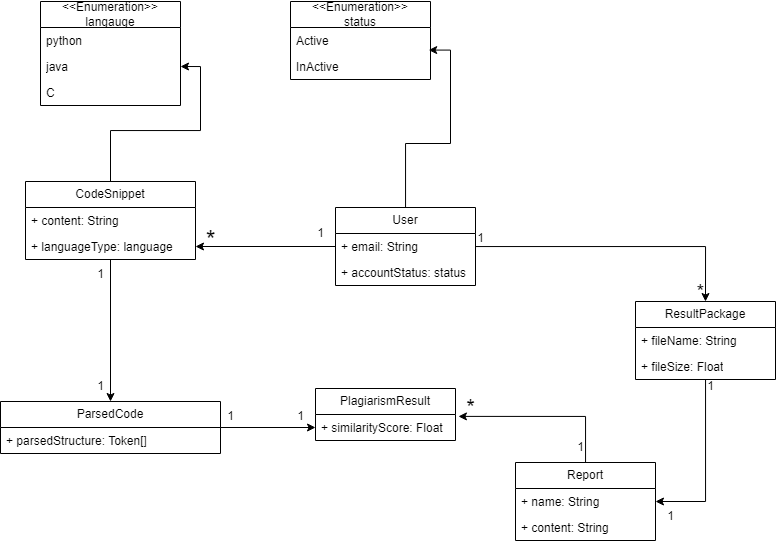
\includegraphics[height=.58\textheight]{./assets/UML.png}
\captionof{figure}{Business Data Model}
\subsection{Data Dictionary}

\textbf{Enums}

\textbf{language}: Represents the programming language used in a code snippet.
\begin{itemize}
    \item \textbf{Values}:
    \begin{itemize}
        \item \texttt{Python}
        \item \texttt{Java}
        \item \texttt{C}
    \end{itemize}
\end{itemize}

\textbf{Classes}

\textbf{CodeSnippet}: Represents the code snippet submitted by a user.
\begin{itemize}
    \item \textbf{Attributes}:
    \begin{itemize}
        \item \texttt{content: String} -- The actual content of the code.
        \item \texttt{languageType: language} -- The programming language used, selected from the \texttt{language} enum.
        \item \texttt{submissionTime: String} -- The timestamp when the code was submitted.
    \end{itemize}
    \item \textbf{Relationships}:
    \begin{itemize}
        \item A \texttt{User} can submit multiple \texttt{CodeSnippet} objects (1-to-many relationship).
        \item Each \texttt{CodeSnippet} generates exactly one \texttt{ParsedCode} (1-to-1 relationship).
    \end{itemize}
\end{itemize}

\textbf{ParsedCode}: Represents the parsed structure of a code snippet for analysis.
\begin{itemize}
    \item \textbf{Attributes}:
    \begin{itemize}
        \item \texttt{parsedStructure: Token[]} -- An array of tokens that represents the parsed structure of the code. Note: the actual structure of tokens hasn't been determined yet.
    \end{itemize}
    \item \textbf{Relationships}:
    \begin{itemize}
        \item Each \texttt{CodeSnippet} is associated with exactly one \texttt{ParsedCode}.
        \item Each \texttt{ParsedCode} generates exactly one \texttt{PlagiarismResult} (1-to-1 relationship).
    \end{itemize}
\end{itemize}

\textbf{PlagiarismResult}: Represents the outcome of the plagiarism detection process.
\begin{itemize}
    \item \textbf{Attributes}:
    \begin{itemize}
        \item \texttt{timeStamp: String} -- The timestamp of when the plagiarism result was generated.
        \item \texttt{similarityScore: Float} -- The similarity score between the code snippet and other submissions.
    \end{itemize}
    \item \textbf{Relationships}:
    \begin{itemize}
        \item A \texttt{ParsedCode} generates exactly one \texttt{PlagiarismResult} (1-to-1 relationship).
        \item A \texttt{PlagiarismResult} can be part of one \texttt{ResultPackage} (many-to-one relationship).
    \end{itemize}
\end{itemize}

\textbf{ResultPackage}: Represents a zipped file that contains one or more plagiarism results, which can be sent via email.
\begin{itemize}
    \item \textbf{Attributes}:
    \begin{itemize}
        \item \texttt{fileName: String} -- The name of the result package file.
        \item \texttt{fileSize: Float} -- The size of the result package file.
        \item \texttt{timeStamp: String} -- The timestamp of when the result package was generated.
    \end{itemize}
    \item \textbf{Relationships}:
    \begin{itemize}
        \item A \texttt{User} can receive multiple \texttt{ResultPackages} (1-to-many relationship).
        \item Each \texttt{ResultPackage} can include multiple \texttt{PlagiarismResult} objects.
    \end{itemize}
\end{itemize}

\textbf{User}: Represents a user of the system, such as a professor or student.
\begin{itemize}
    \item \textbf{Attributes}:
    \begin{itemize}
        \item \texttt{email: String} -- The email address of the user.
    \end{itemize}
    \item \textbf{Relationships}:
    \begin{itemize}
        \item A \texttt{User} can submit multiple \texttt{CodeSnippet} objects (1-to-many relationship).
        \item A \texttt{User} can receive multiple \texttt{ResultPackages} (1-to-many relationship).
    \end{itemize}
\end{itemize}

\textbf{Relationships Overview}
\begin{itemize}
    \item \texttt{User} submits multiple \texttt{CodeSnippets} (1-to-many).
    \item \texttt{CodeSnippet} is parsed into exactly one \texttt{ParsedCode} (1-to-1).
    \item \texttt{ParsedCode} generates exactly one \texttt{PlagiarismResult} (1-to-1).
    \item \texttt{PlagiarismResult} can be part of one \texttt{ResultPackage} (many-to-one).
    \item \texttt{User} receives multiple \texttt{ResultPackages} (1-to-many).
\end{itemize}



\section{The Scope of the Product}
\subsection{Product Boundary}
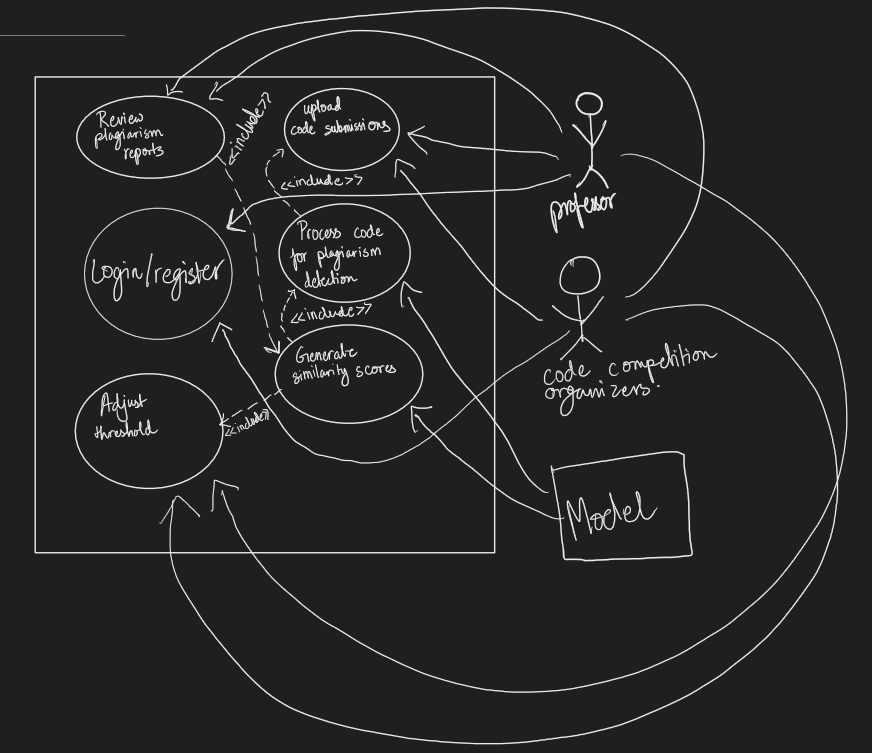
\includegraphics[height=.78\textheight]{assets/UseCase.png}
\captionof{figure}{Use Case Diagram}
Note: The Model here represents our NLP model, which is the core of our product.

\subsection{Product Use Case Table}
\begin{tabular}{ | p{3cm} | p{3cm} | p{3cm} | p{3cm} | }
\hline
\textbf{PUC No} & \textbf{PUC Name} & \textbf{Actor/s} & \textbf{Input/Output} \\ \hline
1 & Upload Code Submissions & Professor, Competition Organizers & Code Submission (in) / Uploaded Code (out) \\ \hline
2 & Process Code for Plagiarism Detection & Model & Uploaded Code (in) / Processed Code (out) \\ \hline
3 & Generate Similarity Scores & Model & Processed Code (in) / Similarity Scores (out) \\ \hline
4 & Review Plagiarism Reports & Professor, Competition Organizers & Similarity Scores (in) / Plagiarism Report (out) \\ \hline
5 & Adjust Plagiarism Detection Threshold & Professor, Competition Organizers & Threshold Input (in) / Updated Threshold (out) \\ \hline
6 & Login/Register & Professor, Competition Organizers & Login Credentials (in) / Access to System (out) \\ \hline
\end{tabular}
\captionof{table}{Product Use Case Table}

\subsection{Individual Product Use Cases (PUC's)}
\textbf{PUC 1: Upload Code Submissions}\\
\textbf{Actors:} Professor, Competition Organizers\\
\textbf{Preconditions:} The user is logged in and has the necessary permissions to upload submissions.\\
\textbf{Main Scenario:}
\begin{enumerate}
    \item The system prompts the user to upload code files.
    \item The user uploads the required code files and submits them.
    \item The system stores the submitted files for plagiarism detection processing.
    \item The system notifies the user that the upload was successful.
\end{enumerate}
\textbf{Postconditions:} The code submissions are available for plagiarism detection.\\[0.2cm]

\textbf{PUC 2: Process Code for Plagiarism Detection}\\
\textbf{Actors:} Model, Professor\\
\textbf{Preconditions:} Code submissions have been uploaded and are ready for processing.\\
\textbf{Main Scenario:}
\begin{enumerate}
    \item The system retrieves the submitted code for processing.
    \item The system parses the code to generate structured representations (e.g., Abstract Syntax Tree or AST, still TBD for our use).
    \item The system compares the parsed code against other uploaded submissions and datasets using the plagiarism detection model.
    \item The system stores the processed results for similarity scoring.
\end{enumerate}
\textbf{Postconditions:} The code is fully processed and ready for generating similarity scores.\\[0.2cm]

\textbf{PUC 3: Generate Similarity Scores}\\
\textbf{Actors:} Model\\
\textbf{Preconditions:} The code has been processed and structured.\\
\textbf{Main Scenario:}
\begin{enumerate}
    \item The system calculates similarity scores by comparing the structured code.
    \item The system generates detailed similarity reports with scores for each code submission.
    \item The system emails the similarity reports in a .zip file to the user.
\end{enumerate}
\textbf{Postconditions:} Similarity scores are available for review.\\[0.2cm]

\textbf{PUC 4: Review Plagiarism Reports}\\
\textbf{Actors:} Professor, Competition Organizers\\
\textbf{Preconditions:} Similarity scores have been generated and are ready for review.\\
\textbf{Main Scenario:}
\begin{enumerate}
    \item The professor/organizer logs into the system and uploads the .zip file containing the plagiarism reports.
    \item The system displays the plagiarism reports, including similarity scores and flagged submissions.
    \item The professor/organizer reviews the results and flags any cases for investigation or further action.
    \item The system logs any flags or notes made by the professor/organizer.
\end{enumerate}
\textbf{Postconditions:} The professor/organizer has reviewed the plagiarism reports.\\[0.2cm]

\textbf{PUC 5: Adjust Plagiarism Detection Threshold}\\
\textbf{Actors:} Professor, Competition Organizers\\
\textbf{Preconditions:} The plagiarism detection system has been configured with default thresholds.\\
\textbf{Main Scenario:}
\begin{enumerate}
    \item The professor/organizer navigates to the plagiarism detection settings.
    \item The system displays the current thresholds for flagging plagiarism.
    \item The professor/organizer adjusts the thresholds based on the desired sensitivity level.
    \item The system applies the new threshold settings to future plagiarism checks.
\end{enumerate}
\textbf{Postconditions:} The new threshold settings are saved and used for subsequent plagiarism checks.\\[0.2cm]

\textbf{PUC 6: Login/Register}\\
\textbf{Actors:} Professor, Competition Organizers\\
\textbf{Preconditions:} The user has an account or needs to register.\\
\textbf{Main Scenario:}
\begin{enumerate}
    \item The user navigates to the login or registration page.
    \item The system prompts the user to enter their credentials (or create a new account).
    \item The user provides the necessary information (email, password, etc.) for login or registration.
    \item The system verifies the credentials or creates a new account.
    \item The system logs the user in or confirms successful registration.
\end{enumerate}
\textbf{Postconditions:} The user is logged into the system and can access the functionalities based on their role.

\section{Functional Requirements}
\subsection{Functional Requirements}
\begin{itemize}
    \item \textbf{FR-1}: The system shall allow code snippets to be
    uploaded into itself.
    \item \textbf{FR-2}:The system shall output similarity scores alongside 
    thresholds that indicate whether or not plagiarism is present within the input
    \item \textbf{FR-3}: The system shall be able to output documentation explaining
    how to interpret any other output (guide document)
    \item \textbf{FR-4}: The system shall allow code snippets to be flagged after similarity
    scores and thresholds are generated
    \item \textbf{FR-5}: The system shall provide a set of similarity scores for all code 
    snippet pairings
    \item \textbf{FR-6}: The system shall allow a report to be created after scores and 
    thresholds are generated that summarize all system outputs 
    \item \textbf{FR-7}: The system will allow users to create an account with an email and password
    \item \textbf{FR-8}: The system will allow users to sign into a created account with 
    their email and password
    \item \textbf{FR-9}: The system shall be able to email all outputs as a .zip file 
    to an email selected by the user
    \item \textbf{FR-10}: System shall be able to visualize a .zip file containing its outputs
    uploaded by user the on the user interface
\end{itemize}

\section{Look and Feel Requirements}

\subsection{Appearance Requirements}
The user interface (UI) must adhere to the following appearance guidelines:
\begin{itemize}
    \item \textbf{LF-AR1: Consistency}: The UI should maintain a uniform color palette, 
    font, and layout across all screens and elements. For instance, the primary 
    color is defined as blue (\#0047AB) for buttons, links, and headers, and 
    white (\#FFFFFF) for background areas.
    
    \item \textbf{LF-AR2: Clarity}: All icons, buttons, and menus should be intuitive and 
    clearly identifiable. Hovering over icons will provide tooltips with a brief 
    description of their functionality.
    
    \item \textbf{LF-AR3: Responsiveness}: The layout should adjust according to screen 
    size, ensuring the interface remains usable on a range of devices, including 
    desktops, tablets, and mobile phones.
\end{itemize}

\subsection{Style Requirements}
The style guidelines for the interface are as follows:
\begin{itemize}
    \item \textbf{LF-SR1: Typography}: The font family used across the UI will be 
    \textit{Roboto}. Headers should use a 24px font size, body text should be 
    14px and button text should be 16px.
    
    \item \textbf{LF-SR2: Color Scheme}: Buttons and interactive elements should use the 
    primary color \#0047AB. Background areas will use \#F0F0F0, and error 
    messages will be highlighted in \#FF0000.
    
    \item \textbf{LF-SR3: Button Styles}: All buttons should have rounded corners with 
    a radius of 5px. On hover, the button background will lighten by 20\%.
    
    \item \textbf{LF-SR4: Spacing and Padding}: There should be at least 10px of padding 
    between elements and a margin of 20px around each section to maintain a clean 
    layout.
\end{itemize}


\section{Usability and Humanity Requirements}

\subsection{Ease of Use Requirements}
The system should be intuitive and simple to use for the target audience.
\begin{itemize}
    \item \textbf{UH-E1: Minimal Learning Curve}: Users should be able to complete tasks 
    with minimal instruction or training, taking at most 5 minutes from start 
    to finish. The interface must guide users intuitively through this process.
    
    \item \textbf{UH-E2: Task Efficiency}: Common tasks should be achievable in no more 
    than three clicks or interactions from the main screen.
    
    \item \textbf{UH-E3: Clear Navigation}: All navigation elements should be labeled 
    clearly and positioned consistently across different pages to avoid confusion.
\end{itemize}

\subsection{Personalization and Internationalization Requirements}
The system will support a customizable experience in the future, but users will 
not be able to modify key settings such as themes or layout preferences at launch.
\begin{itemize}
    \item \textbf{UH-PI1: Future Customization Support}: Future updates will allow users 
    to modify settings such as themes and layouts to suit their personal preferences.
    
    \item \textbf{UH-PI2: English Language Support}: The system will operate exclusively 
    in English, with all dates, currency, and numeric formats adhering to 
    English (US) standards.
\end{itemize}

\subsection{Learning Requirements}
The system should provide clear documentation and onboarding materials.
\begin{itemize}
    \item \textbf{UH-L1: Onboarding}: A guided onboarding process should be available 
    for new users, helping them understand the main features of the system 
    in under 5 minutes.
    
    \item \textbf{UH-L2: Help Documentation}: Detailed help documentation and tooltips 
    should be available for key features to reduce the need for external 
    assistance.
\end{itemize}

\subsection{Understandability and Politeness Requirements}
The system should use clear language and maintain a polite tone in all 
interactions with users.
\begin{itemize}
    \item \textbf{UH-UP1: Clear Language}: All messages and labels should be in simple, 
    everyday language to ensure clarity for users of different levels of 
    technical expertise.
    
    \item \textbf{UH-UP2: Politeness}: Error messages and prompts should be worded 
    politely and offer constructive guidance. Example error messages include:
    \begin{itemize}
        \item \textit{“Oops! Something went wrong. Please try again or contact 
        support if the issue persists.”}
        \item \textit{“We're sorry, but the file you uploaded is not supported. 
        Please upload a .py file.”}
    \end{itemize}
\end{itemize}

\subsection{Accessibility Requirements}
Due to time constraints, the system will not be fully accessible at launch. But this can be a future goal.

\section{Performance Requirements}
\subsection{Speed and Latency Requirements}
\begin{itemize}
    \item \textbf{PR-SL1}: The system should take 10 minutes at most to process 
    and return plagiarism results when given process 500 code snippets of 200 
    lines or less (expected size of course classroom or code competition).
    \item \textbf{PR-SL2}: The system must notify users if processing surpasses ten minutes.
\end{itemize}
\subsection{Safety-Critical Requirements}
There are no safety-critical requirements except for those imposed by our 
precision and accuracy requirements \hyperlink{subsection.12.3}{PR-PA1 and PR-PA2}.
\subsection{Precision or Accuracy Requirements}
\begin{itemize}
    \item \textbf{PR-PA1}: At the default thresholds provided, the system should 
    have an accuracy rate of at least 90\% for identifying plagiarized content.
    \item \textbf{PR-PA2}: At the default thresholds provided, the false positive 
    rate (incorrectly flagged plagiarism cases) must be kept below 5\%.
\end{itemize}
\subsection{Robustness or Fault-Tolerance Requirements}
\begin{itemize}
    \item \textbf{PR-RFT1}: The system will not crash in the case of a malformed input, and will instead issue an error message to the user.
\end{itemize}
\subsection{Capacity Requirements}
\begin{itemize}
    \item \textbf{PR-C1}: The system should be able to handle batches of inputs without the total processing time exceeding 600 seconds.
\end{itemize}
\subsection{Scalability or Extensibility Requirements}
\begin{itemize}
    \item \textbf{PR-SE1}: The system should be designed in a way such that adding support for new file types or coding languages should not impede current functionality
\end{itemize}
\subsection{Longevity Requirements}
\begin{itemize}
    \item \textbf{PR-L1}: Backwards compatibility must be maintained when new features are introduced
    \item \textbf{PR-L2}: The system should be designed such that the natural language processing part can be changed in accordance with new research in the field.
\end{itemize}

\section{Operational and Environmental Requirements}
\subsection{Expected Physical Environment}
There are no specific physical environment requirements for our product since it is entirely software-based.
Users can access the tool from any location with an internet connection via a web browser on any major operating system.

\subsection{Wider Environment Requirements}
There are no wider environment requirements for our product since it operates entirely within a virtual environment.
Because of this, environmental factors are outside of the scope of our project.

\subsection{Requirements for Interfacing with Adjacent Systems}
\begin{itemize}
    \item \textbf{OE-IAS1}: The system will provide the option to interface with cloud computing (AWS, Azure) 
    \item \textbf{OE-IAS2}: The system will deploy the frontend and backend code in a free hosting Service
    \item \textbf{OE-IAS3}: The system will use external services for user authentication 
\end{itemize}
\subsection{Productization Requirements}
For the tool to be ready for widespread use, it should meet several productization requirements:
\begin{itemize}
    \item \textbf{OE-P1: User-friendly interfaces} for professors and code contest administrators, allowing easy input and clear, actionable outputs.
    \item \textbf{OE-P2: Documentation and training materials} to help users understand how to utilize the tool effectively, including explanations of how the similarity scores are calculated and how to interpret them.
    \item \textbf{OE-P3: Scalability}, ensuring that the tool can handle many code submissions simultaneously without performance degradation.
\end{itemize}

\subsection{Release Requirements}
To release the tool effectively, certain conditions must be met:
\begin{itemize}
    \item \textbf{OR-R1: Beta testing} with a select group of professors and students to gather feedback on usability, performance, and false positive/negative rates.
    \item \textbf{OR-R2: Clear versioning} and change logs to track improvements over time, particularly as new programming languages or detection features are added.
    \item \textbf{OR-R3: Ongoing support}, including the ability to update the plagiarism detector with new models or features as they are developed.
\end{itemize}

\section{Maintainability and Support Requirements}
\subsection{Maintenance Requirements}
\begin{itemize}
    \item \textbf{MS-M1: Versioning}: Keep track of and store model versions to allow
     switches between experimental models and previous versions. A verifiable metric is 
     that version history exists.

    Justification: Gives the ability to work on separate model architectures to try 
    improvements in different directions as well as rollback on model releases 
    if something goes wrong as well as provide experimental releases.
    
    \item \textbf{MS-M2: Metric Reports}: Every model release shall be accompanied by 
    a report of metrics decided upon to track model performance. A verifiable metric is 
    that the report exists.

    Justification: Gives clarity on whether the model is being improved or not and what
     specific changes may be damaging the model. This will allow model health and 
     performance to be tracked and maintained over time.

    \item \textbf{MS-M3: Issue Tracking}: Every bug should be registered in an issue-tracking system. A verifiable metric is bugs existing as issues. 

    Justification: Brings attention to what bugs have been resolved and which 
    ones still require work.
    
\end{itemize}
\subsection{Supportability Requirements}
\begin{itemize}
    \item \textbf{MS-S1: Documentation}: provide concise (max 30 lines) comments on 
    all APIs and algorithms used in the code base. This will allow others to 
    comprehend what sections may need updates or bug fixes A verifiable metric is 
    comment exists at every piece of API code or algorithm.
    
    Justification: leaves no obfuscation in where somebody should adjust 
    code or update a component by clarifying what responsibility each area
     of code holds.

    \item \textbf{MS-S2: Logging}: provides a report of code components that 
    executed leading up to a crash whenever a crash occurs, so bugs can 
    be identified and fixes can be staged. A verifiable metric is a log with relevant 
    information about the crash, such as a stack trace, is generated for the user 
    to view when a crash occurs.

    Justification: Almost 100\% necessary for effectively debugging issues in
     the code and giving the ability to support the model in the future for 
     people who aren't familiar with the code base.

    \item \textbf{MS-S3: Community Acknowledgement}: provide a pathway for users to post
     or vote for requests/issues that should be addressed. A verifiable metric is the existence
      of said pathway, like email or GitHub issues or forum.

    Justification: Will highlight to the community what are current pain points 
    that should be prioritized and communication about how it is desired to 
    address them.

\end{itemize}
\subsection{Adaptability Requirements}
\begin{itemize}
    \item \textbf{MS-A1: Dataset Compatibility}: provide compatibility for at least 
    two data formats when it comes to training datasets. A verifiable metric is that data 
    the formats that are accepted.

    Justification: will allow the model to accommodate a wider amount of datasets 
    and provides it better longevity in case either one of its data formats 
    becomes less popular.
    
    \item \textbf{MS-A2: Template Adherence}: Every model layer/component follows a 
    template. A verifiable metric is that a template exists for all model layers/components and
     is upheld by said layers/components.

    Justification - if somebody wishes to update the model with new 
    layers/components or modify existing ones, there will be a guide to make 
    the process straightforward and encourage those conducting the update to 
    follow through.

    \item \textbf{MS-A3: Modularity}:  every model layer/component can be treated as 
    an individual function. A verifiable metric is that model layers/components can be fed an 
    input and produce an output which reflects only operations conducted within
     the layer/component.

    Justification - enables removal or substitution of individual model 
    layers/components which may be problematic or less efficient, similar to 
    how one may remove or substitute a function in a program, without having to
     overhaul a larger/more significant portion of the model architecture.


\end{itemize}

\section{Security Requirements}
\subsection{Access Requirements}
\begin{itemize}
    \item \textbf{SR-A1: Authentication}: The system shall require user authentication
    before allowing access to the tool. Only authenticated users can upload code for comparison.

    Justification - Users need to be identifiable so that they can receive their results via email and so that usage limits can be imposed upon them.
\end{itemize}

\subsection{Integrity Requirements}
Integrity requirements are outside the scope of this project. The system is designed to avoid storing any user data.
Since no data is retained, data integrity is not a concern.

\subsection{Privacy Requirements}
\begin{itemize}
    \item \textbf{SR-P1: Zero Data Retention}: The system shall retain no user-uploaded data beyond the immediate need of the task.
    Refer to requirement CR-SC5 for more information.

    Justification - This ensures user privacy and protects sensitive academic work from being mishandled.

    \item \textbf{SR-P2: In Transit Encryption}: All data (including code snippets) shall be encrypted while being uploaded to or downloaded
    from the system using secure encryption protocols.

    Justification - Protecting user data during transmission ensures that it can't be intercepted by unauthorized third parties.
\end{itemize}

\subsection{Audit Requirements}
\begin{itemize}
    \item \textbf{SR-AD1: Auditable Logs}: The system shall log all user interactions and actions (such as authentication events, code uploads, and plagiarism checks) anonymously, without storing user-uploaded code or sensitive data.

    Justification - While no user data is retained, logging system events and user actions provide a transparent way to track system usage and ensure accountability without violating the zero data retention policy.
\end{itemize}

\subsection{Immunity Requirements}
Immunity requirements are beyond the scope of this project. The system should not need to defend against external attacks
beyond the security measures already in place (e.g., authentication, encryption).
The focus of the project is on code plagiarism detection, and immunity against malicious actors is not a primary concern.

\section{Cultural Requirements}
\subsection{Cultural Requirements}
No major cultural requirements are identified for this project but some that could be taken into consideration are:\\ \\ 
\noindent \textbf{Data Privacy and Ethical Use}\\ 
\textbf{Student Privacy}: In some cultures and institutions, the handling of student work and data is highly regulated. Laws like the FIPPA mandate strict data privacy standards. The system should ensure that student data, including their code submissions, is securely handled, anonymized where possible, and not stored unnecessarily.
\\ \\
\noindent \textbf{Differences in Academic Integrity Norms}\\ 
\textbf{Varying Definitions of Plagiarism}: Some cultures and institutions promote collaboration and code borrowing so it is essential to define what plagiarism is in the context of this project. The tool should also be modifiable in its threshold for detecting plagiarism so institutions can change it to their needs.


\section{Compliance Requirements}

In developing the enhanced plagiarism detection tool, it is imperative to address
various compliance requirements to ensure the tool operates legally, ethically,
and in alignment with industry standards. These requirements encompass legal
obligations related to data protection, intellectual property rights, and
adherence to educational policies, as well as compliance with established software
development and data security standards.

\subsection{Legal Requirements}

\begin{enumerate}
    \item \textbf{CR-L1: Data Protection and Privacy Laws}: The tool will process sensitive
    information, including students' code submissions, which may be considered personal
    data under Canadian privacy laws such as the \textit{Personal Information Protection 
    and Electronic Documents Act} (PIPEDA) at the federal level, and Ontario's \textit{Freedom of 
    Information and Protection of Privacy Act} (FIPPA) for public institutions. Compliance with these 
    laws require:
    \begin{itemize}
        \item \textbf{Lawful Basis for Data Processing}: Ensuring that the collection and use of 
        personal information is authorized under PIPEDA or FIPPA, typically requiring consent from 
        students before processing their code or ensuring that processing is necessary for educational purposes.
        \item \textbf{Data Minimization and Purpose Limitation}: Collecting only the data
        necessary for plagiarism detection and using it solely for that purpose.
        \item \textbf{Transparency and Information Rights}: Informing students about how
        their data will be used, stored, and protected, and respecting their rights to
        access, correct, or withdraw their personal information.
        \item \textbf{Security Measures}: Implementing appropriate technical and
        organizational measures to safeguard personal data against unauthorized access,
        loss, or disclosure, as required under PIPEDA and FIPPA.
    \end{itemize}

    \item \textbf{CR-L2: Intellectual Property Rights}: Under the \textit{Copyright Act} of Canada, 
    students typically hold the intellectual property rights to their original code. 
    The tool must:
    \begin{itemize}
        \item \textbf{Respect Ownership}: Use students' code exclusively for plagiarism
        detection without unauthorized distribution or reproduction.
        \item \textbf{Establish Clear Terms}: Provide clear terms of service or agreements
        outlining how the code will be used, ensuring students are aware and consent to
        these terms.
        \item \textbf{Avoid Infringement}: Ensure that any storage or processing of code
        does not violate the \textit{Copyright Act} or institutional policies.
    \end{itemize}

    \item \textbf{CR-L3: Academic Integrity Policies}: The tool must align with the academic
    integrity and misconduct policies of Canadian educational institutions by:
    \begin{itemize}
        \item \textbf{Supporting Fair Evaluation}: Assisting educators in identifying
        potential plagiarism accurately without bias.
        \item \textbf{Due Process}: Ensuring that students have the opportunity to respond
        to plagiarism accusations, with results from the tool serving as part of a broader
        investigation rather than definitive proof.
        \item \textbf{Confidentiality}: Maintaining the confidentiality of students' work
        and any findings related to plagiarism investigations.
    \end{itemize}
\end{enumerate}

\subsection{Standards Compliance Requirements}

\begin{enumerate}
    \item \textbf{CR-SC1: Software Development Standards}: Adherence to recognized software development practices is essential for ensuring quality and maintainability.
        \begin{itemize}
            \item \textbf{SOLID Principles}: The project will follow SOLID principles—Single Responsibility, 
            Open/Closed, Liskov Substitution, Interface Segregation, and Dependency Inversion—to promote clean,
             maintainable, and scalable code.
            \item \textbf{Documentation and Testing}: Thorough documentation will be maintained throughout 
            development, and rigorous testing will be conducted to validate the tool's performance and reliability.
        \end{itemize}



    \item \textbf{CR-SC2: Data Security Standards}: Protecting sensitive data is a priority, and although full 
    compliance with industry security standards such as ISO/IEC 27001 may not be feasible for a student 
    capstone project, we will take measures to ensure data security.
        \begin{itemize}
            \item \textbf{OWASP Guidelines}: Basic security measures will be implemented in line with the 
            Open Web Application Security Project (OWASP) guidelines to mitigate common vulnerabilities such 
            as injection attacks and unauthorized access.
        \end{itemize}


    \item \textbf{CR-SC3: Accessibility Standards}: The tool will be designed to support basic accessibility features.
    \begin{itemize}
        \item \textbf{Screen Reader Support}: Key elements of the user interface will be made compatible with 
        screen readers to assist visually impaired users.
        \item \textbf{Alt Text for Images}: All images and non-text content will include descriptive alt text to 
        improve accessibility for users relying on assistive technologies.
        \item \textbf{Text Color Contrast}: The tool will ensure sufficient contrast between text and background 
        colors to improve readability for users with visual impairments or color blindness.
    \end{itemize}
        

    \item \textbf{CR-SC4: Ethical AI and Machine Learning Standards}: As the tool leverages AI
    technologies, it must adhere to ethical standards in AI development.
    \begin{itemize}
        \item \textbf{Transparency and Explainability}: Ensuring that the AI models used
        are transparent in their operation and that their decision-making processes can be
        explained to users.
        \item \textbf{Fairness and Non-Discrimination}: Preventing biases in the AI models
        that could unfairly target or disadvantage any group of students. Ensuring that names
        and other potentially discriminatory information are not used in the detection process.
    \end{itemize}

    \item \textbf{CR-SC5: Data Handling and Retention Policies}: Establishing clear policies for
    how data is managed throughout its lifecycle.
    \begin{itemize}
        \item \textbf{Zero Data Retention}: No user data will be retained beyond the immediate needs of the task.
        All user-uploaded data will be immediately loaded into memory and subsequently removed from disk as soon
        as the task is finished.
        \item \textbf{Secure Disposal}: Implementing procedures for the secure deletion or
        anonymization of data that is no longer needed.
        \item \textbf{Audit and Compliance}: Regularly auditing data handling practices to
        ensure compliance with all relevant laws and standards.
    \end{itemize}
\end{enumerate}

By meticulously addressing these legal and standards compliance requirements, the
project not only safeguards the rights and interests of all stakeholders but also
enhances the credibility and trustworthiness of the plagiarism detection tool. Ensuring
compliance is fundamental to the tool's success and its acceptance by educational
institutions, educators, and students alike.


\section{Open Issues}
\subsection{System Design Uncertainty}
\begin{itemize}
    \item How the integration of the Natural Language Processing (NLP) model with the code submission system will work. Such as choosing what NLP model to use, how to train it, and where to host it.
    \item Selecting the most appropriate techniques for semantic code analysis, such as Abstract Syntax Trees (ASTs) or vector embeddings.
    \item Deciding on how the model will handle false positives, especially common coding patterns, to avoid misclassification: for instance, students using the same code snippets from a tutorial.
\end{itemize}

\subsection {Data Collection Challenges}
\begin{itemize}
    \item While the project mentions scraping datasets from online programming contests and using pre-labeled datasets, 
    there could be issues with data availability, quality, or ensuring that the data accurately reflects real-world usage.
\end{itemize}

\subsection {Scalability Concerns}
\begin{itemize}
    \item Ensuring the system remains performant when processing large batches of submissions within the 10-minute processing time goal. 
    Handling larger academic institutions with potentially thousands of submissions may challenge the current system's capacity requirements
    \item  Given the limited budget for cloud compute units, it may be challenging to balance performance improvements with cost constraints. 
    If training processes requires more resources than anticipated, costs could quickly escalate.
\end{itemize}
\section{Off-the-Shelf Solutions}
\subsection{Ready-Made Products}

Many ready-made tools aim to detect source-code level plagiarism, the most well-known of which being \href{https://theory.stanford.edu/~aiken/moss/}{MOSS}. MOSS is most commonly used by professors.
There are also a handful of open-source alternatives, including: \href{https://github.com/jplag/JPlag}{JPlag}, \href{https://dickgrune.com/Programs/similarity_tester/}{SIM}, \href{https://warwick.ac.uk/fac/sci/dcs/research/ias/software/sherlock/}{Sherlock}, and \href{https://www.cs.hut.fi/Software/Plaggie/}{Plaggie}.
Most of them support checking multiple languages and use a variety of techniques to improve detection rates. These tools are relatively old and are not all actively developed.

\subsection{Reusable Components}

JPlag uses ANTLR 4 as a parser generator for many of its supported languages. For cross-language support, our tool can reuse JPlag's ANTLR grammar files to create language frontend parsers for each language we choose to support. Using a parser generator with pre-existing grammar files would reduce development time significantly since the alternative would entail writing a custom parser for each supported language. By using ANTLR and JPlag's grammar files, we could feasibly support many source languages as opposed to just one, which would most likely be Python (our product will be written in Python, and Python is capable of parsing its own syntax tree).

\subsection{Products That Can Be Copied}

The primary inspiration for our product is MOSS. Our product, similar to many others, will copy the general data pipeline of input source code. Specifically, after reading an input source code file, plagiarism checkers typically have parsing, tokenizing, and normalizing steps. This is followed by some analysis on the normalized text - \href{https://theory.stanford.edu/~aiken/publications/papers/sigmod03.pdf}{MOSS uses "Winnowing"}, an algorithm that produces local fingerprints in a piece of text.

To reduce development time, we plan to copy the first step (the text preprocessing as described above) of the data pipeline implemented in MOSS. This kind of text normalization is commonly studied and there are many resources that explain implementation details.

\section{New Problems}
\subsection{Effects on the Current Environment}
\begin{itemize}
    \item \textbf{Blind Trust in the Tool}: One potential issue is that users may develop a sense of over-reliance on the tool based solely on the fact that it is AI-based. This can lead to blind trust in its results. This could cause professors to forego manual checks, resulting in incorrect classifications.
\end{itemize}

\subsection{Effects on the Installed Systems}
There should be no new problems for users of this tool since they don't need to install any software on their local machines. The tool's interface is accessed by a web browser, and the processing happens on the server side.

\subsection{Potential User Problems}
\begin{itemize}
    \item \textbf{Difficulty with the New UI}: Some users may struggle to navigate the new UI, resulting in misuse of the tool. Additionally, some settings may not be known by the user and left at their default value, which may cause confusion or result in a worse detection rate.

    \item \textbf{Misinterpretation of Results}: Users may incorrectly interpret the significance of the results provided by the tool. For instance, a high similarity score might be misinterpreted as definitive proof of plagiarism when there could be legitimate reasons for the similarity, such as the use of common libraries or design patterns.
\end{itemize}

\subsection{Limitations in the Anticipated Implementation Environment That May Inhibit the New Product}
\begin{itemize}
    \item \textbf{Limited Compute Power Causing Delays}: If the system is deployed in environments with limited computational resources, such as local servers with insufficient processing power or memory, users may experience longer waiting times for results. Additionally, high computational demands may overload the system during peak usage times, also resulting in longer waiting times.
\end{itemize}

\subsection{Follow-Up Problems}
\begin{itemize}
    \item \textbf{Server Maintenance and Costs}: Long-term maintenance of the server infrastructure could present challenges, including server downtime, performance degradation, and increasing operational costs as more users adopt the system. Costs related to server hosting, cloud processing, and ensuring uptime can grow as demand increases.
    
    \item \textbf{Model Upgrades and Performance Regressions}: Updating or training new models may introduce performance regressions or unexpected behaviour in the plagiarism detection system. For example, a newer model may detect plagiarism more accurately but at the cost of higher processing times or an increase in false positives.
\end{itemize}



\section{Tasks}
\subsection{Project Planning}
\begin{enumerate}
    \item \textbf{Hazard Analysis (October 12 - October 23)}
    \begin{itemize}
        \item \textbf{High-Level Description:} This document identifies potential risks or hazards in the project, assesses their severity,
         and proposes mitigations. It is important to ensure safety and compliance with standards.
        \item \textbf{Story Points:} 12 days
        \item \textbf{Tasks:} Brainstorming hazards, analysis, and review.
    \end{itemize}

    \item \textbf{V\&V Plan (Revision 0) (October 24 - November 1)}
    \begin{itemize}
        \item \textbf{High-Level Description:} The Verification and Validation (V\&V) plan outlines the strategy for ensuring that the system
         is both built correctly and performs as intended. It covers the methods and resources required for testing.
        \item \textbf{Story Points:} 7 days
        \item \textbf{Tasks:} Define tests, acceptance criteria, and procedures for verification and validation.
    \end{itemize}

    \item \textbf{Prep for Proof of Concept Demonstration (November 2 – November 11)}
    \begin{itemize}
        \item \textbf{High-Level Description:} Preparation for a demonstration showing that the core concepts of the system are feasible. 
        It typically involves implementing and testing essential features and preparing to showcase them to stakeholders.
        \item \textbf{Story Points:} 10 day
        \item \textbf{Tasks:} Development of key features and preparation for the demo.
    \end{itemize}

    \item \textbf{Proof of Concept Demonstration (TBD)}
    \begin{itemize}
        \item \textbf{High-Level Description:} A demonstration showing that the core concepts of the system are feasible. This involves 
        implementing and testing essential features and demonstrating them to stakeholders.
        \item \textbf{Story Points:} 1 day
        \item \textbf{Tasks:} Execution and presentation of the demo.
    \end{itemize}

    \item \textbf{Design Document (Revision 0) (November 23 - January 15)}
    \begin{itemize}
        \item \textbf{High-Level Description:} This document outlines the architecture, components, data flow, and design decisions for the system. 
        It serves as a blueprint for the development team.
        \item \textbf{Story Points:} 7 days
        \item \textbf{Tasks:} Detailed system design, architecture planning, and review.
    \end{itemize}

    \item \textbf{Prep for Revision 0 Demonstration (January 16 – February 3)}
    \begin{itemize}
        \item \textbf{High-Level Description:} Preparation for the Revision 0 Demo, which demonstrates functionality that meets the initial design and requirements.
        \item \textbf{Story Points:} 8 days
        \item \textbf{Tasks:} Prepare, refine, and finalize core product features.
    \end{itemize}

    \item \textbf{Revision 0 Demonstration (Date: TBD)}
    \begin{itemize}
        \item \textbf{High-Level Description:} A demonstration of the system after the first iteration, showing functionality that meets the initial design and requirements.
        \item \textbf{Story Points:} 1 day
        \item \textbf{Tasks:} Present the system, and showcase its core features.
    \end{itemize}

    \item \textbf{V\&V Report (Revision 0) (February 15 - March 7)}
    \begin{itemize}
        \item \textbf{High-Level Description:} This documents the process of verifying that the system meets its functional and nonfunctional requirements and validating that 
        the system performs as intended. It includes the evaluation of both functional and non-functional requirements, details of unit testing, automated testing, and code 
        coverage metrics. The report also highlights any changes made due to testing and traces these changes back to both requirements and modules. Comparisons to existing 
        implementations are provided, where applicable.
        \item \textbf{Story Points:} 5 days
        \item \textbf{Tasks:} Collect results, analyze tests, and create the report.
    \end{itemize}

    \item \textbf{Final Demonstration (Revision 1) (Date: TBD)}
    \begin{itemize}
        \item \textbf{High-Level Description:} A final demonstration showcasing the complete system. By this stage, the system should be fully functional, meeting all requirements and passing validation.
        \item \textbf{Story Points:} 10 days
        \item \textbf{Tasks:} Ensure all components work seamlessly and prepare the final demo.
    \end{itemize}

    \item \textbf{EXPO Demonstration (April TBD)}
    \begin{itemize}
        \item \textbf{High-Level Description:} This is a public or stakeholder-facing presentation of the system, potentially at an event or exhibition. The focus is on clear communication and showcasing the system’s capabilities.
        \item \textbf{Story Points:} 7 days
        \item \textbf{Tasks:} Practice, set up, and run the demo smoothly.
    \end{itemize}

    \item \textbf{Final Documentation (Revision 1) (Due: April 2)}
    \begin{itemize}
        \item \textbf{High-Level Description:} This is the comprehensive final documentation, which includes all deliverables like the problem statement, development plan, POC plan, requirements document, design, and more.
        \item \textbf{Story Points:} 12 days
        \item \textbf{Tasks:} Complete, revise, and polish all components of the documentation.
    \end{itemize}

\end{enumerate}
\subsection{Planning of the Development Phases}
\section*{Phase 1: Proof of Concept (Oct 12 - Nov 11)}
\begin{itemize}
    \item \textbf{Model Development:}
    \begin{itemize}
        \item Story Points: 30 days
        \item Concentrate on training and evaluating the plagiarism detection model. Experiment with various algorithms and techniques.
        \item Weekly Iterations: Regularly assess model performance, making adjustments based on results. Document findings and refine methods to enhance the model's accuracy.
    \end{itemize}
\end{itemize}

\section*{Phase 2: Initial System Design and UI Development (Nov 12 - Feb 3)}
\begin{itemize}
    \item \textbf{Model Development:}
    \begin{itemize}
        \item Story Points: 30 days
        \item Continue refining the model based on insights from the POC. Prepare the model for integration with the overall system architecture.
        \item Mid-January: Finalize the model for production use.
    \end{itemize}

    \item \textbf{UI Development:}
    \begin{itemize}
        \item Begin designing the user interface. Focus on mockups and user experience workflows based on expected model outputs.
        \item Weekly Check-Ins: Collaborate with the model development team to ensure UI designs align with the model's capabilities and outputs.
        \item \textbf{Tasks and Duration:}

        \begin{tabular}{|c|p{4cm}|p{4cm}|p{4cm}|}
            \hline
            \textbf{Task} & \textbf{Estimated Days} & \textbf{Notes} \\
            \hline
            Account Creation UI & 2 & Interface for user registration \\
            \hline
            Comparison UI & 20 & Displaying similarity results \\
            \hline
            Report Generation UI & 10 & Generating and downloading reports \\
            \hline
        \end{tabular}
        \captionof{table}{UI Development Tasks}
    \end{itemize}

    \item \textbf{Unit and Integration Testing:}
    \begin{itemize}
        \item Story points: 5 days
        \item Conduct unit and integration tests between the finalized model and the backend components. Ensure data flow and output processing are functioning correctly.
    \end{itemize}
\end{itemize}

\section*{Phase 3: Final Completion (Feb 4 - Mar 24)}
\begin{itemize}
    \item \textbf{Final Model Tweaks:}
    \begin{itemize}
        \item Make any last-minute adjustments to the model based on integration testing feedback.
    \end{itemize}

    \item \textbf{Backend Development:}
    \begin{itemize}
        \item Develop the backend infrastructure, including user account management and result delivery systems.
        \item \textbf{Tasks and Duration:}

        \begin{tabular}{|c|p{4cm}|p{4cm}|p{4cm}|}
            \hline
            \textbf{Task} & \textbf{Estimated Days} & \textbf{Notes} \\
            \hline
            Account Management & 1 & Handling user registrations and logins \\
            \hline
            Similarity Processing & 14 &  Processing model outputs for similarity scores \\
            \hline
            Report Generation & 7 & Generating reports based on model output \\
            \hline
            Report Delivery & 4 & Sending reports via email \\
            \hline
        \end{tabular}
        \captionof{table}{Backend Development Tasks}
    \end{itemize}

    \item \textbf{UI Finalization:}
    \begin{itemize}
        \item Story points: 10 days
        \item Finalize the UI based on integration testing results and feedback from the model. Ensure all user functionalities are ready for testing.
    \end{itemize}

    \item \textbf{Final Testing and Debugging:}
    \begin{itemize}
        \item Story points: 10 days
        \item Conduct comprehensive testing of the entire system, focusing on functionality, performance, and user experience. Address any bugs and finalize documentation.
    \end{itemize}
\end{itemize}

\section{Migration to the New Product}
\subsection{Requirements for Migration to the New Product}
The migration to the new code plagiarism detection system must be carefully planned and executed to ensure smooth adoption by academic institutions. The following requirements should be addressed:
\begin{itemize}
    \item \textbf{User Training and Support}: Provide comprehensive documentation and training materials for professors, system administrators, and students to familiarize them with the new system. This includes tutorials on how to upload code, interpret results, and resolve flagged cases.
    \item \textbf{Phased Rollout}: Implement a phased migration plan, starting with pilot tests in a controlled environment (e.g., one course or department) before full-scale implementation across the institution.
    \item \textbf{Data Security Compliance}: Ensure data migrations comply with data protection regulations, such as Canada's Privacy Act.
    \item \textbf{System Downtime Minimization}: Plan the migration to minimize downtime and disruption to academic workflows. Ideally, the transition should occur during a break period, when student and faculty activity is low.
\end{itemize}
\subsection{Data That Has to be Modified or Translated for the New System}
For the migration to the new plagiarism detection system, certain data from the legacy systems must be modified or translated to ensure compatibility:
\begin{itemize}
    \item \textbf{Code Submissions}: Legacy code submissions must be translated into a format that the new system can process, especially if the old system uses proprietary formats or different programming language encoding.
    \item \textbf{User Permissions}: Any user and administrator accounts need to be transferred to the new system. This includes roles, permissions, and access levels.
    \item \textbf{Configuration Data}: Settings from the old system, such as threshold scores, course configurations, and institution-specific policies, must be mapped and adjusted to fit the new system’s configuration parameters.
    \item \textbf{Metadata and Logs}: Metadata (e.g., anonymous submission timestamps, course IDs) and system logs related to prior plagiarism checks should be preserved and transferred, ensuring transparency and continuity.
\end{itemize}

\section{Costs}
The costs associated with this project come from several different parts of the project.
\begin{itemize}
    \item Data must be acquired before training the model. The data required to
    train the model can cost money. However, the team intends to automate
    processes to acquire data, and thus there is no charge incurred. An unknown
    amount of money will be needed for data if the team's method of acquiring
    data fails.
    \item In the training and testing phase, the model will require hardware to
    be trained on. The team intends to use Google Co-lab and leverage the
    hardware provided by their cloud platform. This will cost approximately 30
    dollars for the required computation. However, if more training and testing
    is required, more Google compute units will be used, costing more money. An
    upper limit of 150 dollars is set, which is 5 times more than the current
    guess. 
    \item The front end will need to be hosted somewhere. However, free
    alternatives exist, thus this will have no cost incurred.

\end{itemize}
In total, the project should only cost approximately 30 dollars. The cost is
subject to change, and can increase/decrease depending on the amount of data
needed, and how much Google's cloud hardware is used.

\section{User Documentation and Training}

\subsection{User Documentation Requirements}
The user documentation must be comprehensive, detailing all functionalities of the system. It should include step-by-step guides for professors, system administrators, and competition organizers, ensuring they can:
\begin{itemize}
    \item Upload code submissions for plagiarism checks.
    \item Understand the process behind similarity score generation.
    \item Review and interpret similarity reports.
    \item Adjust plagiarism detection thresholds to suit specific needs.
    \item Administer the system, including managing users, system settings, and troubleshooting common issues.
\end{itemize}

The documentation should also include a frequently asked questions (FAQ) section, covering common user issues, and should be available in both written and video tutorial formats.

\subsection{Training Requirements}
The system requires training sessions for all primary users, including professors, competition organizers, and system administrators. Training should focus on:
\begin{itemize}
    \item How to upload and submit code for plagiarism checking.
    \item How to review and interpret similarity scores and plagiarism reports.
    \item Techniques for flagging plagiarism cases and overriding false positives.
    \item Administrative training for system administrators, covering user management, and system maintenance.
    \item Ongoing support for users, including refresher training and updates on new features as the system evolves.
\end{itemize}

Training materials should be available in multiple formats: in-person workshops, webinars, and self-paced online courses.


\section{Waiting Room}
It is too early in the project to have a waiting room. This section will be completed as the project progresses and new features are considered.

\section{Ideas for Solution}
It is too early in the project to have ideas for solutions. This section will be completed as the project progresses.

\newpage{}
\section*{Appendix --- Reflection}

The information in this section will be used to evaluate the team members on the
graduate attribute of Lifelong Learning.  Please answer the following questions:

\begin{enumerate}
  \item What knowledge and skills will the team collectively need to acquire to
  successfully complete this capstone project?  Examples of possible knowledge
  to acquire include domain-specific knowledge from the domain of your
  application, or software engineering knowledge, mechatronics knowledge or
  computer science knowledge.  Skills may be related to technology, or writing,
  or presentation, or team management, etc.  You should look to identify at
  least one item for each team member.
  \textbf{Knowledge Areas:}
    \begin{itemize}
        \item \textbf{Language normalization}: Understanding source-code level processing techniques necessary for transforming input text into a format usable by NLP models.
        \item \textbf{NLP Techniques}: Understanding and applying Natural Language Processing (NLP) techniques to analyze code submissions. Necessary to develop algorithm/model project will rely on at its core.
        \item \textbf{Server Deployment}: Understanding how to deploy algorithm/model in conjunction with UI to receive 
        requests for analyzing plagiarism from a non-local user. Necessary to be able to host our model outside of a local host.
    \end{itemize}
    \textbf{Skills:}
    \begin{itemize}
        \item \textbf{Writing}: The ability to convey thoughts in a formalized manner. This is necessary to write documentation for projects such as SRS.
        \item \textbf{Team Management}: The ability to delegate responsibilities amongst members in a respectful manner while working off feedback from teammates about their enjoyment of given tasks to retain a cohesive team dynamic. This is necessary to keep work on track and maintain an enthusiastic team spirit.
        \item \textbf{Proactive Communication}: Letting others know in advance the direction you want to head in for a given task. This is necessary to allow strong planning that will not crumble under roadblocks in code development, which are bound to happen.
    \end{itemize}
    \textbf{Julian}: Server Deployment, Proactive Communication \\
    \textbf{Lucas}: NLP Techniques, Team Management \\
    \textbf{Dennis}: NLP Techniques, Team Management \\
    \textbf{Mohammad}: NLP Techniques, Writing, Proactive Communication
  \item For each of the knowledge areas and skills identified in the previous
  question, what are at least two approaches to acquiring the knowledge or
  mastering the skill?  Of the identified approaches, which will each team
  member pursue, and why did they make this choice?
    \begin{itemize}
        \item \textbf{Server Deployment}: YouTube Videos, Online Articles, Building miniproject
        \item \textbf{Proactive Communication}: Scheduling Meetings for direction, Notebook Reminders
        \item \textbf{Language normalization}: YouTube Videos, Research Papers, Open source code on GitHub
        \item \textbf{NLP Techniques}: YouTube Videos, Online Articles, Research Papers
        \item \textbf{Team Management}: YouTube Videos, Online Articles, GitHub Project Management Tools
        \item \textbf{Writing}: Writing Documentation, Online Articles
        \item \textbf{Proactive Communication}: Notebook Reminders, Scheduling Meetings
    \end{itemize}
    Which team member chose to pursue which approach, and why?
    \begin{itemize}
        \item \textbf{Lucas Chen:} 
        \begin{itemize}
            \item \textbf{NLP Techniques}: Lucas will pursue YouTube videos and online reading to understand NLP techniques. This is because he learns best through visual and auditory methods.
            \item \textbf{Team Management}: Lucas will pursue learning more about GitHub project management tools and techniques. This is because he has taken on the role of project manager and needs to understand how to manage the team effectively.
        \end{itemize}
        \item \textbf{Dennis Fong:}
        \begin{itemize}
            \item \textbf{NLP Techniques}: Dennis will look for research papers on NLP, especially ones that pertain to the topic of this project. This is because he seeks a deeper understanding of the inner workings of a NLP model from both a math and code perspective.
            \item \textbf{Team Management}: Dennis will learn about team management through the use of GitHub and the many features it supports for managing a project for the team. He is not as familiar with GitHub as his team members, and this will serve as a strong learning experience.
        \end{itemize}

        \item \textbf{Julian Cecchini:} 
        \begin{itemize}
            \item \textbf{Server Deployment}: Julian will pursue online articles to learn this. He finds maintaining attention for long YouTube videos can be cumbersome and if he's interrupted, it's easier to find where he left off in online articles compared to YouTube videos. Also, he doesn't feel he has time to trial server deployment in as a side project. He lacks experience in server deployment compared to the rest of the team, so he seeks to close the knowledge gap to be able to contribute and gain experience in this area.

            \item \textbf{Proactive Communication}: Julian will schedule meetings for thought direction on given tasks. He feels the commitment imposed by a meeting where he must announce his thoughts will have him try more consistently to announce his mind's direction than a notebook reminder that suggests he should bring some thoughts forward. He feels its essential he masters this while dealing with multiple extracurriculars on top of capstone so he doesn't lose touch with the team.
        \end{itemize}

        \item \textbf{Mohammad Mohsin Khan:}
        \begin{itemize}
            \item \textbf{NLP Techniques}: Mohammad will pursue online articles and research papers to understand NLP techniques. This is because he prefers to read and analyze information at his own pace.
            \item \textbf{Writing}: Mohammad will practice writing by creating documentation for the project. This hands-on approach will help him improve his writing skills through practical application.
            \item \textbf{Proactive Communication}: Mohammad will use notebook reminders to prompt him to communicate proactively. This method aligns with his preference for written reminders and will help him stay organized and on track.
        \end{itemize}
        
        \item \textbf{Luigi Quattrociocchi:}
        \begin{itemize}
            \item \textbf{Language normalization}: Luigi will study open-source repositories on GitHub and read research papers relating to source-code-level language processing. This knowledge will be critical to transforming user input into a format that is usable for NLP analysis. This choice was made because Luigi has many ideas for the implementation of these techniques and he believes that formalizing this will help the project proceed.
            \item \textbf{Server Deployment}: Luigi aims to improve his knowledge of server deployment and general web development best practices and techniques by watching YouTube videos and participating in discussions with the team about how we plan to deploy the system. Luigi finds that he lacks expertise in this area and would like to contribute to this aspect of the project.
            \item \textbf{Writing}: Luigi will pursue improvement in writing by continuing to write documentation and enforcing strict linter rules about comments and function docstrings in the project source code. This will help him improve his communication with his team and improve documentation for any other maintainers of the project.
        \end{itemize}
    \end{itemize}
\end{enumerate}

\end{document}